% !TeX root = RJwrapper.tex
\title{corVis: An R Package for Visualising Associations and Conditional
Associations}
\author{by Amit Chinwan and Catherine Hurley}

\maketitle

\abstract{%
Correlation matrix displays are important tools to explore multivariate
datasets. These displays with other measures of association can
summarize interesting patterns to an analyst and assist them in framing
questions while performing exploratory data analysis. In this paper, we
present new visualisation techniques to visualise association between
all the variable pairs in a dataset in a single plot, which is something
existing displays lack. Also, we propse new methods to visualise
relationship among variable pairs using conditioning. We use different
layouts like matrix or linear for our displays. We use seriation in our
displays which helps in highlighting interesting patterns easily. The R
package \texttt{corVis} provides an implementation.
}

\hypertarget{section-1-introduction}{%
\section{Section 1: Introduction}\label{section-1-introduction}}

Correlation matrix display helps in visually exploring correlations
among variables during Exploratory Data Analysis (EDA) of a multivariate
dataset. Popularized by \citet{friendly2002corrgrams} as corrgram, these
displays are produced by first calculating the correlation among the
variables and then plotting these calculated values in a matrix display.
With effective ordering techniques, these displays quickly highlight
variables which are highly correlated and an analyst interested in
building a predictive model could use these displays to flag and avoid
multicollinearity.

The correlation displays are generally used with Pearson's correlation
coefficient and are therefore limited to quantitative variables. An
analyst can use one-hot encoding of the qualitative variables in order
to use these displays but will need to deal with the high dimensions as
a result of the encoding. In addition to the dimensionality problem, it
is not easy to assess the overall correlation when using the one-hot
encoding.

Tukey and Tukey \citep{tukey1985computer} introduced scagnostics which
are diagnostic measures, quantifying density, shape, trend, and other
features, of a scatterplot. Along with scagnostics, they proposed a
scagnostics scatterplot matrix which is a visual display to explore and
compare these measures for all the variable pairs in a dataset. By
comparing multiple measures at once, variable pairs with high difference
among measures could be identified and looked at in more detail. In a
similar manner, a display comparing association measures will help in
finding interesting variable pairs. Many association measures have been
proposed to summarize different types of relationships. The most
commonly used measure is Pearson's correlation coefficient which
captures any linear trend present between the variables. Other popular
measures include Kendall's or Spearman's rank correlation coefficient
which are non-parametric measures and look for monotonic relationship.
Distance correlation \citep{szekely2007measuring} is an important
measure useful in exploring non-linear relationships. The information
theory measure maximal information coefficient (MIC)
\citep{reshef2011detecting} is capable of summarizing complex
relationships. With an effective displaying technique for the multiple
measures of association, it will be easier to .

Small multiples (or Trellis display) is a simple yet powerful approach
to compare partitions of data and understand multidimensional datasets
\citep{tufte1986thevisual}. The display is produced by splitting the
data into groups by a conditioning variable and then plotting the data
for each group. Such displays allow analysts to quickly infer about the
impact of the conditioning variable. A similar idea applied to displays
of association measures (correlation plot) will help uncover underlying
patterns in the data. One such pattern is Simpson's paradox which can be
detected by comparing Pearson's correlation for data at overall level
versus individual levels of the conditioning variable.

In this paper, we propose extensions of the correlation plot and new
visualizations which look at variables of mixed type, multiple
association measures and conditional associations. These displays are
implemented in the R package \CRANpkg{corVis}. The next section provides
a review of existing packages which deal with correlation displays and a
quick background on association measures and the packages used for
calculating them. Then we describe our approach to calculate the
association measures, followed by visualizations of associations and
conditional associations. We conclude with a summary and future work.

\hypertarget{section-2-background}{%
\section{Section 2: Background}\label{section-2-background}}

In this section we provide a brief review of existing packages used for
correlation displays and association measure calculation.

\hypertarget{section-2.1-literature-review-on-correlation-displays}{%
\subsection{Section 2.1: Literature Review on Correlation
Displays}\label{section-2.1-literature-review-on-correlation-displays}}

According to \citet{hills1969looking}, ``the first and sometimes only
impression gained by looking at a large correlation matrix is its
largeness''. To overcome this, \citet{murdoch1996graphical} proposed a
display for large correlation matrices which uses a matrix layout of
ellipses where the parameters of the ellipses are scaled to the
correlation values. \citet{friendly2002corrgrams} expanded on this idea
by rendering correlation values as shaded squares, bars, ellipses, or
circular `pac-man' symbols. The variables in the matrix displays were
optionally ordered using the angular ordering of the first two eigen
vectors of the correlation matrix. The ordering places highly-correlated
pairs of variables nearby, making it easier to quickly identify groups
of variables with high mutual correlation.

Nowadays, there are many R packages devoted to correlation
visualisation. Table \ref{tab:corrdisplay-packages} provides a summary,
listing the displays offered, and whether these extend to factor
variables or mixed numeric-factor pairs.

The R package \CRANpkg{corrplot} \citep{corrplot2021} provides an
implementation of the methods in \citet{friendly2002corrgrams}. The
package \CRANpkg{corrr} \citep{corrr2020} organises correlations as tidy
data, so leveraging the data manipulation and visualisation tools of the
\CRANpkg{tidyverse} \citep{tidyverse}. In addition to various matrix
displays, the package offers network displays where line-thickness
encodes correlation magnitude, with a filtering option to discard
low-correlation edges.

The package \CRANpkg{corrgrapher} \citep{corrgrapher} uses a network
plot for exploring correlations, where the nodes close to each other
have high correlation magnitude, edge thickness encodes the absolute
correlation value and edge color indicates the sign of correlation. The
package also handles mixed type variables by using association measures
obtained as transformations of \(p\)-values obtained from Pearson's
correlation test in the case of two numeric variables, Kruskal's test
for numerical and factor variables, and a chi-squared test for two
categorical variables.

The package \CRANpkg{linkspotter} \citep{linkspotter} offers a variety
of association measures (distance correlation, MIC, maximum normalized
mutual information) in addition to correlation, where the measure used
depends on whether the variables are both numerical, categorical or
mixed. The results are visualized in a network plot, which may be
packaged into an interactive shiny application.

Our own package \CRANpkg{corVis} offers a variety of displays, and has
new features not available elsewhere, in particular simultaneous display
of multiple association measures, and association displays stratified by
levels of a grouping variable. This will be described in the following
sections.

There have been other extensions to correlation displays which are
useful when dealing with high dimensional datasets.
\citet{hills1969looking} proposed a QQ plot of the \(z\)-transform of
the entries of the correlation matrix to discover correlation
coefficients too large to come from a normal distribution with mean
zero. \citet{buja2016visualization} proposed Association Navigator which
is an interactive visualization tool for large correlation matrices with
upto 2000 variables. The R package \CRANpkg{scorrplot} \citep{scorr}
produces an interactive scatterplot for exploring pairwise correlations
in a large dataset by projecting variables as points on a scatterplot
with respect to some user-selected variables of interest, driven by a
geometric interpretation of correlation and encoding the correlation as
vertical gridlines in the plot. The package allows user to update
variable of interest which creates tour of the correlation space between
different projections of the data.

The R package \CRANpkg{correlationfunnel} offers a novel display which
assists in feature selection in a setting with a single response and
many predictor variables. All numeric variables including the response
are binned. All (now categorical) variables in the resulting dataset are
one-hot encoded and Pearson's correlation calculated with the response
categories. The correlations are visualised in a dot-plot display, where
predictors are ordered by maximum correlation magnitude. Correlations
between one-hot encoded variables are challenging to interpret,
especially as the number of levels increase. In corVis we offer a
similar dot-plot display, but showing multiple correlation or
association measures, or alternatively measures stratified by a grouping
variable.

\begin{Schunk}
\begin{table}

\caption{\label{tab:corrdisplay-packages}List of the R packages dealing with correlation or correlation displays with information on whether the plots display multiple measures, conditional display of measures and mixed variables in a single plot}
\centering
\begin{tabular}[t]{lll}
\toprule
Package & Display & MixedVariables\\
\midrule
corrplot & heatmap & \\
corrr & heatmap/network & \\
corrgrapher & network & \\
linkspotter & network & Yes\\
correlation & heatmap/network & \\
\addlinespace
corVis & heatmap/matrix/linear & Yes\\
\bottomrule
\end{tabular}
\end{table}

\end{Schunk}

\hypertarget{section-2.2-literature-review-on-association-measures}{%
\subsection{Section 2.2: Literature Review on Association
Measures}\label{section-2.2-literature-review-on-association-measures}}

An association measure is defined as a numerical summary quantifying the
relationship between two or more variables. The measure is called
symmetric if its value is invariant to the choice of independent or
dependent variable during the calculation. For example, Pearson's
correlation coefficient summarizes the strength and direction in the
range \([-1,1]\) of the linear relationship present between two numeric
variables and is symmetric. Kendall's or Spearman's rank correlation
coefficient are other popular measures which assess monotonic
relationship in interval \([-1,1]\) among two numeric variables and are
symmetric measures.

Pearson's correlation is the most popular association measure because of
its easier calculation and interpretability but its limitations such as
influence of outliers on its value and measuring only linear
dependencies makes it a less useful measure of association overall. The
recent measures such as distance correlation
\citep{szekely2007measuring} and MIC \citep{reshef2011detecting}
overcome these limitations and are more suitable for datasets with both
linear and non-linear patterns.

\begin{Schunk}
\begin{figure}

{\centering 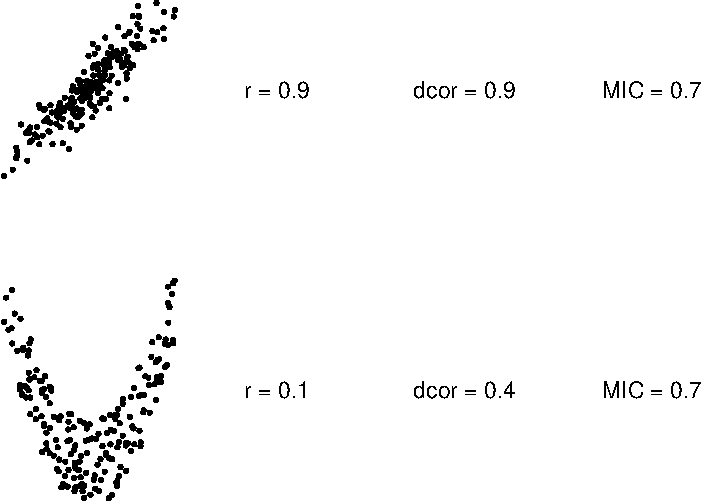
\includegraphics{rj_paper_files/figure-latex/motivation-patterns-1} 

}

\caption[Multiple association measures for simulated linear and non-linear pattern]{Multiple association measures for simulated linear and non-linear pattern. The first row of the plot shows a linear pattern, the value of Pearson's correlation, distance correlation and MIC. The second row of the plot shows a non-linear pattern along with the values for association measures. All three association measures show a high value for the linear relationship and hence are useful for linear patterns. For the non-linear pattern, distance correlation and MIC are more suitable measures than Pearson's correlation.}\label{fig:motivation-patterns}
\end{figure}
\end{Schunk}

Figure \ref{fig:motivation-patterns} shows a plot of simulated linear
and non-linear patterns. The first row shows a linear relationship along
with the value for measures such as Pearson's correlation, distance
correlation and maximal information coefficient respectively for the
pattern. In a similar manner, the second row shows a quadratic
relationship and its values for Pearson's correlation, distance
correlation and maximal information coefficient respectively.\\
It is clearly evident from Figure \ref{fig:motivation-patterns} that all
the three measures summarizes the pattern with linear relationship quite
well. For the non-linear pattern, distance correlation and MIC are
better in detecting underlying relationship than Pearson's correlation.
This suggests that association measures such as distance correlation,
MIC and other measures should be used along with Pearson's correlation
for exploring relationships among variables in the datasets where there
is no prior knowledge about the possible patterns in the data.

The distance correlation coefficient \citep{szekely2007measuring} is an
association measure which looks for any relationship among two numeric
variables using the distances between observations of these variables
and summarizes the relationship in \([0,1]\). The distance correlation
is \(0\) only when the variables are independent and is a symmetric
measure.

The maximal information coefficient (MIC) \citep{reshef2011detecting} is
an information theory measure which uses mutual information among the
two variables for its calculation. The main idea is to find a grid out
of possible grids on a scatterplot of two numeric variables, in order to
discretize the variables, which maximises the mutual information for the
two variables. A normalisation technique is used to make the mutual
information from different grids comparable. Referred as `a correlation
of 21st century' \citep{speed2011correlation}, MIC is capable of
summarizing different types of relationships, not just linear or
monotonous, between numeric variables and is in range \([0,1]\).
\citet{reshef2011detecting} used MIC and other related statistics to
explore pairwise relationships in large data sets such as major-league
baseball, gene expression, global health, and the human gut microbiota.

Both distance correlation and MIC have advantages of detecting
non-linear and complex relationship but these measures aren't perfect
yet. \citet{commentSimonTibshirani} showed that distance correlation has
more statistical power than MIC. Also, distance correlation is not an
approximation when compared to MIC. On the other hand, distance
correlation computation is slower as compared to the conventional
association measures such as Pearson's correlation for datasets with
high number of cases.

In addition to association measures for numeric variables, association
measures for ordinal, nominal and mixed variable pairs are useful in
exploring a multivariate dataset. We now give an overview of available
association measures for other variable types.

\citet{agresti2010analysis} provides an overview of the association
measures which are used for exploring association between ordinal
variables. Kendall's tau-b \citep{kendall1945treatment} is an
association measure useful in summarizing the relationship in range
\([-1,1]\) between two ordinal variables. It is a relatively stable
measure than Goodman and Kruskal's gamma with respect to the changes in
categories of any variable i.e.~if two categories are merged to make a
single category. The polychoric correlation \citep{olsson1979maximum}
measures the correlation between two ordinal variables by assuming two
normally distributed latent variables for a contingency table of two
ordinal variables and summarizes the association in \([-1,1]\).

The association measures for the case of nominal pair of variables
should be invariant to the order in which the categories appear.
Pearson's contingency coefficient uses the \({\chi}^2\) value from the
Pearson's \({\chi}^2\) test for independence and is a useful measure to
summarize the association in \([0,1]\) between two nominal variables.
Another measure for nominal variable pair is the Uncertainty coefficient
\citep{theil1970estimation} measuring the proportion of uncertainty in
one variable which is explained by the other variable. The uncertainty
coefficient measure is in the range \([0,1]\) and is not symmetric.

\hypertarget{section-3-introducing-corvis}{%
\section{Section 3: Introducing
corVis}\label{section-3-introducing-corvis}}

\CRANpkg{corVis} is an R package which calculates measures of
association for every variable pair in a dataset and provides
visualizations for displaying associations. Most of the existing
correlation displays are limited to numeric pairs of variables. This
package extends these displays to every variable pair. The main goal of
our work is to propose displays for multiple association measures and
conditional associations display which are useful for uncovering
interesting patterns in the data. This will help in identifying variable
pairs which shows a type of relationship or pattern in a dataset with
large number of variables.

While designing these displays we consider matrix and linear layouts. A
matrix layout reduces the effort in looking up for variable pairs
corresponding to a cell or panel, and different measures may be
displayed on the upper and lower triangle of the matrix. On the other
hand, the filtering of variable pairs, for example pairs having measure
value greater than a threshold, is easier with linear layouts in
comparison to matrix layouts.

Table \ref{tab:function-corVis} provides a list of the functions
available in the package. The functions \texttt{calc\_assoc} and
\texttt{calc\_assoc\_all} are responsible for calculating association
measures which are used as input for the \texttt{plot\_assoc\_matrix}
and \texttt{plot\_assoc\_linear} functions. The functions
\texttt{plot\_assoc\_matrix} and \texttt{plot\_assoc\_linear} produces
association display, multiple association measures display and
conditional association display, in a matrix and linear layout
respectively. We provide detailed examples on calculation and
visualisation of association and conditional association in next
sections.

\begin{Schunk}
\begin{table}

\caption{\label{tab:function-corVis}List of functions in corVis package}
\centering
\begin{tabular}[t]{>{}lll}
\toprule
Function & Usage & Description\\
\midrule
\textbf{calc\_assoc} & Calculation & Calculates association measures\\
\textbf{calc\_assoc\_all} & Calculation & Calculates all the association measures available in package\\
\textbf{plot\_assoc\_matrix} & Visualization & Visualize assocition and conditional association in matrix plot\\
\textbf{plot\_assoc\_linear} & Visualization & Visualize assocition and conditional association in linear plot\\
\textbf{show\_assoc} & Visualization & Association (or conditional) plot for a pair of variables\\
\bottomrule
\end{tabular}
\end{table}

\end{Schunk}

\hypertarget{section-4-corvis-calculating-association}{%
\section{Section 4: corVis: Calculating
Association}\label{section-4-corvis-calculating-association}}

This section describes the calculation of association measures in our
package \CRANpkg{corVis}. The package provides a standard interface for
calculating a collection of various measures of association which
quantifies the relationship between two variables. The association
measures available in the package are not limited to numeric variables
and are used with nominal, ordinal and mixed variable pairs as well. The
package also provides a functionality for handling missing value or
\texttt{NA} while calculating the association measures.

Table \ref{tab:association-measures} lists different functions provided
in the package to calculate varoius measures of association. The
\texttt{Function} column represents \texttt{tbl\_*} functions which are
used to calculate a single association measure. The \texttt{typeX} and
\texttt{typeY} columns provide the information on types of variables
which can be used with the corresponding functions. The \texttt{X} or
\texttt{Y} variable is one of the numeric, nominal or ordinal type. The
\texttt{from} column corresponds to the external package functions used
to calculate the association measures by \texttt{tbl\_*} functions. The
\texttt{symmetric} column represents if the measure is symmetric i.e.~if
its value doesn't change by the choice of independent or dependent
variable during its calculation. The last column provides the range of
values for these measures. The function \texttt{tbl\_easy} calculates
association measures available in the R package \CRANpkg{correlation}
and is suitable for different variable types.

The functions in Table \ref{tab:association-measures} such as
\texttt{tbl\_ace}, \texttt{tbl\_cancor} and \texttt{tbl\_nmi} which
calculates maximal correlation coefficient, canonical correlationa and
normailzed mutual information respectively, have been implemented in
\CRANpkg{corVis}.

For numeric pairs of variables, the package provides a range of
association measures. The popular correlation coefficients like
Pearson's, Spearman's or Kendall's are calculated using
\texttt{tbl\_cor} function. The measures such as distance correlation or
MIC are calculated using \texttt{tbl\_dcor} or \texttt{tbl\_mine}
respectively. The association measures available in the package for the
ordinal pairs of variables are polychoric correlation and Kendall's
coefficients which are calculated using \texttt{tbl\_polycor} or
\texttt{tbl\_tau} respectively. For nominal pairs of variables, the
functions like \texttt{tbl\_gkTau}, \texttt{tbl\_gkGamma},
\texttt{tbl\_uncertainty}, \texttt{tbl\_chi}, \texttt{tbl\_cancor} are
used for exploring association among the variables.

The function \texttt{tbl\_cancor} calculates a measure of association
based on canonical correlations for mixed pairs of variables. Nominal
variables are converted into sets of dummy variables, which are then
assigned score to find the maximal correlation. For two numeric
variables this measure is identical to absolute correlation, for two
factors the correlation is identical to that obtained from
correspondence analysis.

The functions listed in Table \ref{tab:association-measures} for
calculating association measures provide a functionality for handling
missing value or \texttt{NA} in the dataset. Each of these functions
either have a \texttt{handle.na} argument or automatically uses pairwise
complete observations (depending on the package used for calculation)
for taking care of missing values present in the data.

\begin{Schunk}
\begin{table}

\caption{\label{tab:association-measures}List of the functions available in the package for calculating different association measures along with the packages used for calculation.}
\centering
\resizebox{\linewidth}{!}{
\begin{tabular}[t]{llllll}
\toprule
Function & X & Y & from & symmetric & range\\
\midrule
tbl\_cor & numerical & numerical & stats::cor & Y & {}[-1,1]\\
tbl\_dcor & numerical & numerical & energy::dcor2d & Y & {}[0,1]\\
tbl\_mine & numerical & numerical & minerva::mine & Y & {}[0,1]\\
tbl\_ace & numerical & numerical & corVis & Y & {}[0,1]\\
tbl\_polycor & ordinal & ordinal & polycor::polychor & Y & {}[-1,1]\\
\addlinespace
tbl\_tau & ordinal & ordinal & DescTools::KendalTauA,B,C,W & Y & {}[-1,1]\\
tbl\_gkGamma & ordinal & ordinal & DescTools::GoodmanKruskalGamma & Y & {}[-1,1]\\
tbl\_gkTau & nominal & nominal & DescTools::GoodmanKruskalTau & N & {}[0,1]\\
tbl\_uncertainty & nominal & nominal & DescTools::UncertCoef & Y & {}[0,1]\\
tbl\_chi & nominal & nominal & DescTools::ContCoef & Y & {}[0,1]\\
\addlinespace
tbl\_cancor & nominal/numerical & nominal/numerical & corVis & Y & {}[0,1]\\
tbl\_nmi & nominal & nominal & corVis & Y & {}[0,1]\\
tbl\_easy & nominal/numerical & nominal/numerical & correlation::correlation & Y & {}[-1,1]\\
\bottomrule
\end{tabular}}
\end{table}

\end{Schunk}

\hypertarget{calculating-association-for-a-single-type-of-variable-pairs}{%
\subsection{Calculating association for a single type of variable
pairs}\label{calculating-association-for-a-single-type-of-variable-pairs}}

We have a function which creates a tibble structure for the variable
pairs in a dataset along with calculated association measure. The
package contains various functions (shown in Table
\ref{tab:association-measures}) for different association measures in
the form \texttt{tbl\_*} to calculate them. For example, in order to
calculate distance correlation for numeric pair of variables in a
dataset, the function \texttt{tbl\_dcor} is used.

\begin{Schunk}
\begin{Sinput}
distance <- tbl_dcor(iris)
distance
\end{Sinput}
\begin{Soutput}
#> # A tibble: 6 x 4
#>   x            y            measure measure_type
#>   <chr>        <chr>          <dbl> <chr>       
#> 1 Sepal.Width  Sepal.Length   0.311 dcor        
#> 2 Petal.Length Sepal.Length   0.859 dcor        
#> 3 Petal.Width  Sepal.Length   0.827 dcor        
#> 4 Petal.Length Sepal.Width    0.542 dcor        
#> 5 Petal.Width  Sepal.Width    0.513 dcor        
#> 6 Petal.Width  Petal.Length   0.974 dcor
\end{Soutput}
\end{Schunk}

In the tibble output for the functions mentioned in Table
\ref{tab:association-measures} \texttt{x} and \texttt{y} represents a
pair of variables. The \texttt{measure} variable represents the
calculated value for association measure. And the \texttt{measure\_type}
variable represents the association measure calculated for \texttt{x}
and \texttt{y} pair.

\hypertarget{calculating-association-measures-for-whole-dataset}{%
\subsection{Calculating association measures for whole
dataset}\label{calculating-association-measures-for-whole-dataset}}

\texttt{calc\_assoc} is used to calculate association measures for all
variable pairs in a dataset at once in a tibble structure. The variable
pairs in the output are unique pairs in the dataset where \texttt{x}
\(\neq\) \texttt{y}. Because of the tidy structure of the output, the
data manipulation and visualisation tools of \CRANpkg{tidyverse}
\citep{tidyverse} are applicable and are useful for further exploration
of pairwise associations. In addition to tibble structure, the output
also has \texttt{pairwise} and \texttt{data.frame} class which are
important class attributes for producing visual summaries in this
package.

The function \texttt{calc\_assoc} has a \texttt{types} argument which is
a tibble of the \texttt{tbl\_*} functions for different types of
variable pairs. The default tibble is \texttt{default\_assoc()} which
includes \texttt{tbl\_cor} if both the variables are numeric and
calculates Pearson's correlation , \texttt{tbl\_gkGamma} if both the
variables are ordinal and calculates Goodman and Kruskal's gamma ,
\texttt{tbl\_cancor} if one is factor and other is numeric and
calculates canonical correlation, and canonical correlation for the rest
of the variable pairs.

\begin{Schunk}
\begin{Sinput}
default_measures <- default_assoc()
default_measures
\end{Sinput}
\begin{Soutput}
#> # A tibble: 4 x 4
#>   funName     typeX   typeY   argList
#>   <chr>       <chr>   <chr>   <list> 
#> 1 tbl_cor     numeric numeric <NULL> 
#> 2 tbl_gkGamma ordered ordered <NULL> 
#> 3 tbl_cancor  factor  numeric <NULL> 
#> 4 tbl_cancor  other   other   <NULL>
\end{Soutput}
\begin{Sinput}
iris_assoc <- calc_assoc(d = iris,
                         types = default_measures)
iris_assoc
\end{Sinput}
\begin{Soutput}
#> # A tibble: 10 x 4
#>    x            y            measure measure_type
#>    <chr>        <chr>          <dbl> <chr>       
#>  1 Sepal.Width  Sepal.Length  -0.118 pearson     
#>  2 Petal.Length Sepal.Length   0.872 pearson     
#>  3 Petal.Width  Sepal.Length   0.818 pearson     
#>  4 Species      Sepal.Length   0.787 cancor      
#>  5 Petal.Length Sepal.Width   -0.428 pearson     
#>  6 Petal.Width  Sepal.Width   -0.366 pearson     
#>  7 Species      Sepal.Width    0.633 cancor      
#>  8 Petal.Width  Petal.Length   0.963 pearson     
#>  9 Species      Petal.Length   0.970 cancor      
#> 10 Species      Petal.Width    0.964 cancor
\end{Soutput}
\begin{Sinput}
class(iris_assoc)
\end{Sinput}
\begin{Soutput}
#> [1] "pairwise"   "tbl_df"     "tbl"        "data.frame"
\end{Soutput}
\end{Schunk}

The default tibble of measures is updated using the
\texttt{update\_assoc} function which has arguments for updating the
\texttt{tbl\_*} functions to calculate association measures depending on
the type variable pair in the dataset and a method for \texttt{tbl\_*}
functions which calculates more than one measure. The
\texttt{update\_assoc} function has an argument \texttt{default} which
has the \texttt{default\_assoc()} tibble as its default value and is
useful when \texttt{tbl\_*} functions need to be updated for a few types
of variable pairs.

\begin{Schunk}
\begin{Sinput}
updated_assoc <- update_assoc(default_measures,
                              num_pair = "tbl_cor",
                              num_pair_argList = "spearman",
                              mixed_pair = "tbl_cancor",
                              other_pair = "tbl_nmi")
updated_assoc
\end{Sinput}
\begin{Soutput}
#> # A tibble: 4 x 4
#>   funName     typeX   typeY   argList  
#>   <chr>       <chr>   <chr>   <list>   
#> 1 tbl_cor     numeric numeric <chr [1]>
#> 2 tbl_gkGamma ordered ordered <NULL>   
#> 3 tbl_cancor  factor  numeric <NULL>   
#> 4 tbl_nmi     other   other   <NULL>
\end{Soutput}
\end{Schunk}

\begin{Schunk}
\begin{Sinput}
updated_iris_assoc <- calc_assoc(d = df, 
                                 types = updated_assoc)
updated_iris_assoc
\end{Sinput}
\begin{Soutput}
#> # A tibble: 3 x 4
#>   x           y        measure measure_type
#>   <chr>       <chr>      <dbl> <chr>       
#> 1 Usage       Function   0.647 nmi         
#> 2 Description Function   1     nmi         
#> 3 Description Usage      0.647 nmi
\end{Soutput}
\end{Schunk}

\texttt{calc\_assoc} also has a \texttt{handle.na} argument for handling
the \texttt{NA} or missing values which is fed into the \texttt{tbl\_*}
functions used with the \texttt{types} argument for different types of
variable pairs. The default value is set to \texttt{TRUE} for using
pairwise complete observations for calculating a measure of association
between two variables.

\hypertarget{calculating-multiple-association-measures}{%
\subsection{Calculating multiple association
measures}\label{calculating-multiple-association-measures}}

The multiple association measures are calculated using
\texttt{calc\_assoc\_all} function in the package. The function takes a
dataset and a list of measures as input and outputs a tibble structure
with multiple measures of association for every variable pair. This
output serves as input to the multiple association measures plot
function for comparison of measures for variable pairs.

\begin{Schunk}
\begin{Soutput}
#> # A tibble: 22 x 4
#>    x            y            measure measure_type
#>    <chr>        <chr>          <dbl> <chr>       
#>  1 Sepal.Width  Sepal.Length  -0.118 pearson     
#>  2 Petal.Length Sepal.Length   0.872 pearson     
#>  3 Petal.Width  Sepal.Length   0.818 pearson     
#>  4 Petal.Length Sepal.Width   -0.428 pearson     
#>  5 Petal.Width  Sepal.Width   -0.366 pearson     
#>  6 Petal.Width  Petal.Length   0.963 pearson     
#>  7 Sepal.Width  Sepal.Length   0.118 cancor      
#>  8 Petal.Length Sepal.Length   0.872 cancor      
#>  9 Petal.Width  Sepal.Length   0.818 cancor      
#> 10 Species      Sepal.Length   0.787 cancor      
#> # ... with 12 more rows
\end{Soutput}
\end{Schunk}

\hypertarget{calculating-conditional-association}{%
\subsection{Calculating conditional
association}\label{calculating-conditional-association}}

\texttt{calc\_assoc} is also used to calculate association measures for
all the variable pairs at different levels of a categorical variable.
This helps in exploring the conditional associations and find out the
differences between the groups of the conditioning variable. The
function has a \texttt{by} argument which is used as the grouping
variable and needs to be categorical.

\begin{Schunk}
\begin{Sinput}
iris_assoc_by <- calc_assoc(d = iris,
                            by = "Species")
iris_assoc_by
\end{Sinput}
\begin{Soutput}
#> # A tibble: 24 x 5
#>    x            y            measure measure_type by        
#>    <chr>        <chr>          <dbl> <chr>        <fct>     
#>  1 Sepal.Width  Sepal.Length   0.743 pearson      setosa    
#>  2 Petal.Length Sepal.Length   0.267 pearson      setosa    
#>  3 Petal.Width  Sepal.Length   0.278 pearson      setosa    
#>  4 Petal.Length Sepal.Width    0.178 pearson      setosa    
#>  5 Petal.Width  Sepal.Width    0.233 pearson      setosa    
#>  6 Petal.Width  Petal.Length   0.332 pearson      setosa    
#>  7 Sepal.Width  Sepal.Length   0.526 pearson      versicolor
#>  8 Petal.Length Sepal.Length   0.754 pearson      versicolor
#>  9 Petal.Width  Sepal.Length   0.546 pearson      versicolor
#> 10 Petal.Length Sepal.Width    0.561 pearson      versicolor
#> # ... with 14 more rows
\end{Soutput}
\end{Schunk}

By default, the function \texttt{calc\_assoc} calculates the association
measures for all the variable pairs at different levels of the grouping
variable and the pairwise association measures for the ungrouped data
(\texttt{overall}) when used with the \texttt{by} argument. This
behavior can be changed by setting \texttt{include.overall} argument to
\texttt{FALSE}.

\begin{Schunk}
\begin{Sinput}
iris_assoc_by <- calc_assoc(d = iris,
                            by = "Species",
                            include.overall = FALSE)
iris_assoc_by
\end{Sinput}
\begin{Soutput}
#> # A tibble: 18 x 5
#>    x            y            measure measure_type by        
#>    <chr>        <chr>          <dbl> <chr>        <fct>     
#>  1 Sepal.Width  Sepal.Length   0.743 pearson      setosa    
#>  2 Petal.Length Sepal.Length   0.267 pearson      setosa    
#>  3 Petal.Width  Sepal.Length   0.278 pearson      setosa    
#>  4 Petal.Length Sepal.Width    0.178 pearson      setosa    
#>  5 Petal.Width  Sepal.Width    0.233 pearson      setosa    
#>  6 Petal.Width  Petal.Length   0.332 pearson      setosa    
#>  7 Sepal.Width  Sepal.Length   0.526 pearson      versicolor
#>  8 Petal.Length Sepal.Length   0.754 pearson      versicolor
#>  9 Petal.Width  Sepal.Length   0.546 pearson      versicolor
#> 10 Petal.Length Sepal.Width    0.561 pearson      versicolor
#> 11 Petal.Width  Sepal.Width    0.664 pearson      versicolor
#> 12 Petal.Width  Petal.Length   0.787 pearson      versicolor
#> 13 Sepal.Width  Sepal.Length   0.457 pearson      virginica 
#> 14 Petal.Length Sepal.Length   0.864 pearson      virginica 
#> 15 Petal.Width  Sepal.Length   0.281 pearson      virginica 
#> 16 Petal.Length Sepal.Width    0.401 pearson      virginica 
#> 17 Petal.Width  Sepal.Width    0.538 pearson      virginica 
#> 18 Petal.Width  Petal.Length   0.322 pearson      virginica
\end{Soutput}
\end{Schunk}

The tibble output in the conditional setting has a similar structure as
\texttt{calc\_assoc} used with no \texttt{by} argument. When used with
the \texttt{by} argument, an additional \texttt{by} column representing
the levels of the categorical variable is added to the tibble output.
The \texttt{x} and \texttt{y} variables in the output are repeated for
every level of \texttt{by} variable. In order to have multiple
\texttt{by} variables, the function \texttt{calc\_assoc} is used
multiple times with a different \texttt{by} variable each time and then
the multiple outputs are binded row wise.

\hypertarget{section-5-corvis-visualising-association}{%
\section{Section 5: corVis: Visualising
Association}\label{section-5-corvis-visualising-association}}

This section provides a detailed description of the novel visualisation
techniques proposed in the package \CRANpkg{corVis}. These methods
display association and conditional association for every variable pair
in a dataset in a single plot and show multiple bivariate measures of
association simultaneously. The package includes functions such as
\texttt{plot\_assoc\_matrix} and \texttt{plot\_assoc\_linear} to produce
these displays in matrix and linear layout respectively. In addition,
the package also provides a function \texttt{show\_assoc} to display a
scatterplot for a numeric variable pair input, a box plot for mixed
variable pair input and bar plot for other variable pair input.

We use two datasets to provide illustrative examples. The first dataset
is \texttt{de\_elect} (German Election Data from 2002 and 2005) from
\CRANpkg{zenplots} package which includes numeric variables only. The
German Election dataset provides the information on election results for
two German elections held in 2002 and 2005. The dataset includes \(299\)
constituencies and \(68\) variables providing information on these
constituencies. For our analysis, we use a subset of variables from
German election dataset which are described in Table
\ref{tab:germanelection}. The poor economic performance of the country
was one of the dominant issues during 2002 German election. To analyse
the same, we use variables including vote proportion for three major
parties in 2002 election, population percentages for different age
groups, percentage of employees in different sectors subjected to social
insurance contribution and percentage unemployment.

\begin{Schunk}
\begin{table}

\caption{\label{tab:germanelection}Variable description of a subset of the German election result dataset from 2002 and 2005.}
\centering
\resizebox{\linewidth}{!}{
\begin{tabular}[t]{ll}
\toprule
Variable & Description\\
\midrule
SPD.02 & Proportion of votes for SPD in 2002\\
CDU.CSU.02 & Proportion of votes for CDU/CSU in 2002\\
Gruene.02 & Proportion of votes for Gruene in 2002\\
Pop.18.25 & population between 18 and 25 years old 2002-12-31 (in percent)\\
Pop.25.35 & population between 25 and 35 years old 2002-12-31 (in percent)\\
\addlinespace
Pop.35.60 & population between 35 and 60 years old 2002-12-31 (in percent)\\
Industry & industry employees subject to social insurance contribution (in percent)\\
CTT & commerce, transportation and telecommunication employees subject to social insurance contribution (in percent)\\
Unemployment.03 & unemployment 2003-12-31 (in percent)\\
\bottomrule
\end{tabular}}
\end{table}

\end{Schunk}

\texttt{cdc} (Behavioral survey data) is the second dataset from
\citet{cdc} which includes numeric, nominal and ordered variables. The
dataset is a random sample of 20,000 people from Behavioral Risk Factor
Surveillance System (BRFSS) survey, which is an annual telephonic survey
of 350,000 people, in United States collected by the Centers for Disease
Control and Prevention (CDC) conducted in 2000. The respondents of the
survey are asked questions related to their diet, weekly physical
activity and even their level of health coverage. The goal of the survey
is to identify risk factors in adult population and report the health
trends. The dataset used here has only 9 questions or variables as
compared to the original dataset which includes more than 200
variables.Table \ref{tab:cdcdata} provides a brief description of the
variables in \texttt{cdc} dataset along with the variable type. The
variables \texttt{genhlth}, \texttt{exerany}, \texttt{smoke100} and
\texttt{age} in the dataset were converted to ordinal factors as they
had a natural ordering. \texttt{hlthplan} and \texttt{gender} were
considered as nominal factors for the analysis. During the association
analysis, we found some individuals with very high values for
\texttt{height}, \texttt{weight} and \texttt{wtdesire}, and filtered out
these cases for further analysis.

\begin{Schunk}
\begin{table}

\caption{\label{tab:cdcdata}Variable description of the CDC dataset}
\centering
\resizebox{\linewidth}{!}{
\begin{tabular}[t]{lll}
\toprule
Variable & Description & VariableType\\
\midrule
genhlth & General health, with categories excellent, very good, good, fair, and poor & ordinal\\
exerany & Respondent exercised in the past month with category 0 and 1 & ordinal\\
hlthplan & Respondent has some form of health coverage & nominal\\
smoke100 & Respondent has smoked at least 100 cigarettes in their entire life with category 0 and 1 & ordinal\\
height & Respondent's height in inches & numerical\\
\addlinespace
weight & Respondent's weight in pounds & numerical\\
wtdesire & Respondent's desired weight & numerical\\
age & Respondent's age in categories [18,25], (25,35], (35,60], (60,99] & ordinal\\
gender & Respondent's gender & nominal\\
\bottomrule
\end{tabular}}
\end{table}

\end{Schunk}

\hypertarget{association-plots}{%
\subsection{Association plots}\label{association-plots}}

For association analysis, we start with calculating the default
association measures for the \texttt{cdc} data using
\texttt{calc\_assoc} and then this result is plotted using
\texttt{plot\_assoc\_matrix} in a matrix layout in Figure
\ref{fig:assoc-matrix-cdcdata}.

\begin{Schunk}
\begin{Sinput}
assoc_cdc <- calc_assoc(d = cdcdata)
plot_assoc_matrix(lassoc = assoc_cdc)
\end{Sinput}
\begin{figure}

{\centering 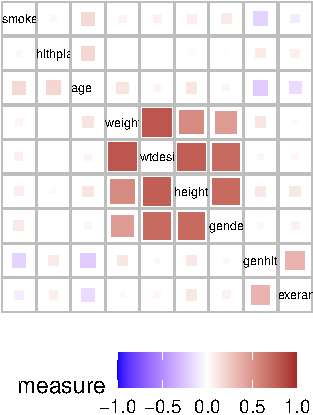
\includegraphics{rj_paper_files/figure-latex/assoc-matrix-cdcdata-1} 

}

\caption[Association matrix display for cdc data showing Pearson's correlation for the numeric variable pairs, Goodman Kruskal's gamma measure for ordered variable pairs, canonical correlation for mixed variable pairs, nominal variable pairs and other variable pairs]{Association matrix display for cdc data showing Pearson's correlation for the numeric variable pairs, Goodman Kruskal's gamma measure for ordered variable pairs, canonical correlation for mixed variable pairs, nominal variable pairs and other variable pairs. The off diagonal cells show the measure value for a variable pair using a square glyph. The color of every square is mapped with the measure value for the variable pair and the area of the square is mapped by absolute measure value for the corresponding variable pair. The plot shows a strong association between desired weight and gender of the indvividuals. Also, there is an negative association between the general health and the age of the individuals suggesting the health of individuals deteriorating with age.}\label{fig:assoc-matrix-cdcdata}
\end{figure}
\end{Schunk}

The diagonal cells in Figure \ref{fig:assoc-matrix-cdcdata} represent
the variables present in the data. Every off diagonal cell contains a
glyph, square in this plot, which is filled with a divergent color scale
representing the value of corresponding association measure for a
variable pair. The \texttt{glyph} argument can be either \texttt{square}
or \texttt{circle}. The area of the square is mapped to absolute value
of the association measure which quickly highlights the associated pairs
of variables. We also offer ordering of the variables in this display so
that highly-associated variables are arranged closer to each other and
the task of detecting patterns or relations becomes easier. The argument
\texttt{var\_order} is used for the variables in the matrix display. The
function uses average linkage hierarchical clustering of the association
matrix of the variables for ordering the variables, which clusters the
highly associated variables together and arranges them nearby.

Figure \ref{fig:assoc-matrix-cdcdata} shows a high positive Pearson's
correlation for (\texttt{wtdesire}, \texttt{height}) which suggests that
taller individuals have higher desired weights. The plot also shows a
negative Goodman Kruskal's gamma measure for the ordered variable pairs
(\texttt{genhlth}, \texttt{age}) and (\texttt{genhlth},
\texttt{smoke100}) indicating that the health of individuals
deteriorates as they age and with more smoking. The positive association
for (\texttt{smoke100}, \texttt{age}) implies that older people tend to
smoke more. Also, it is evident from the plot that individuals who
exercise often are more healthier, shown by the variable pair
(\texttt{exerany}, \texttt{genhlth}).

In order to explore these variable pairs in more detail, the function
\texttt{show\_assoc} is used to plot a scatterplot and a mosaic plot for
numeric and ordinal pairs respectively in Figure
\ref{fig:int-pairs-cdcdata}.

\begin{Schunk}
\begin{Sinput}
show_assoc(d = cdcdata, 
           x = "wtdesire", 
           y = "height")

show_assoc(d = cdcdata, 
           x = "age", 
           y = "genhlth")

show_assoc(d = cdcdata, 
           x = "genhlth", 
           y = "smoke100")

show_assoc(d = cdcdata, 
           x = "smoke100", 
           y = "age")
\end{Sinput}
\begin{figure}
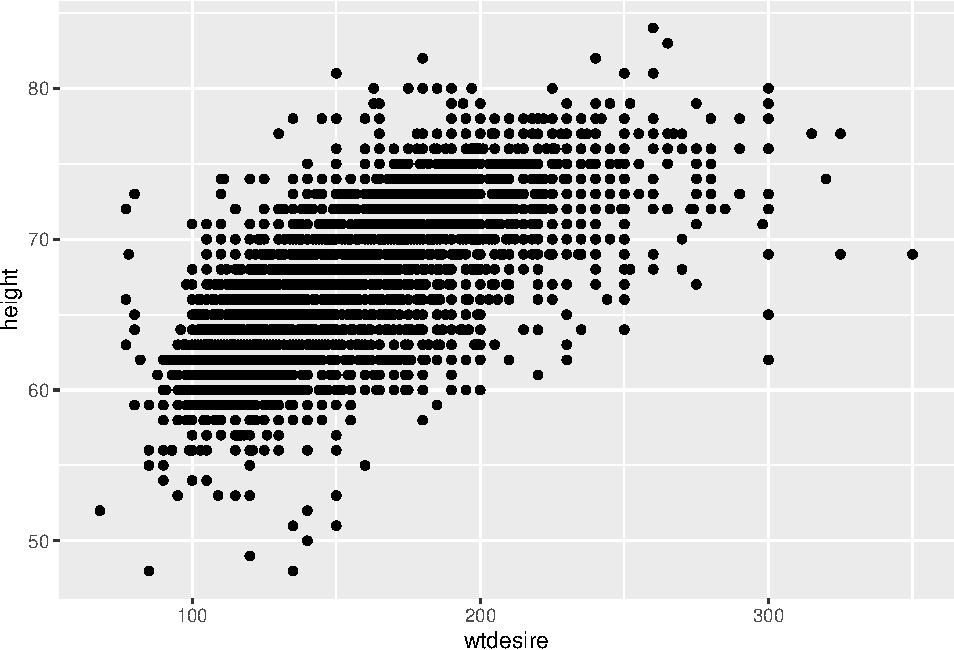
\includegraphics[width=0.5\linewidth]{rj_paper_files/figure-latex/int-pairs-cdcdata-1} 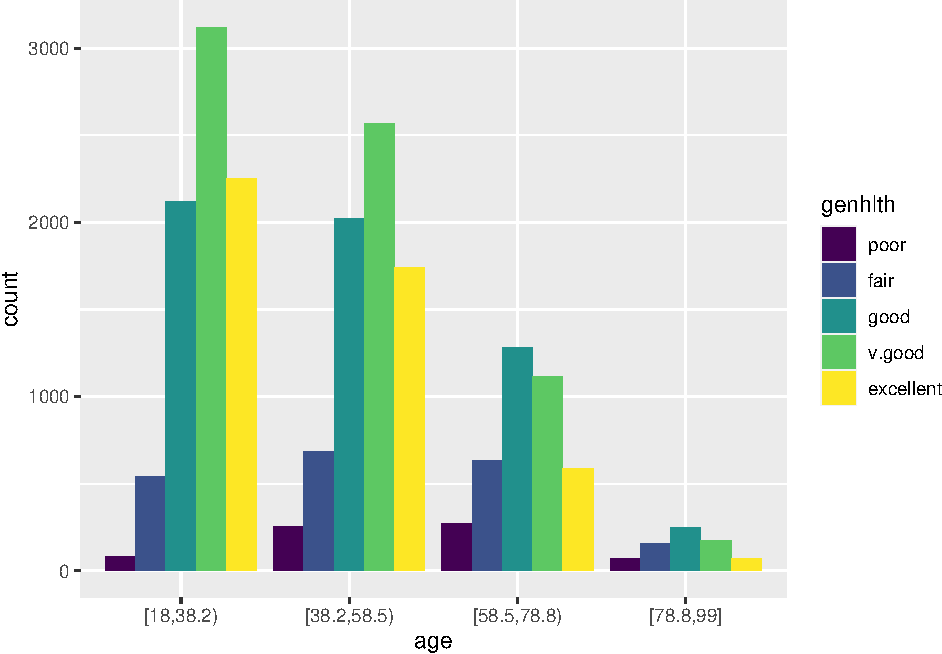
\includegraphics[width=0.5\linewidth]{rj_paper_files/figure-latex/int-pairs-cdcdata-2} 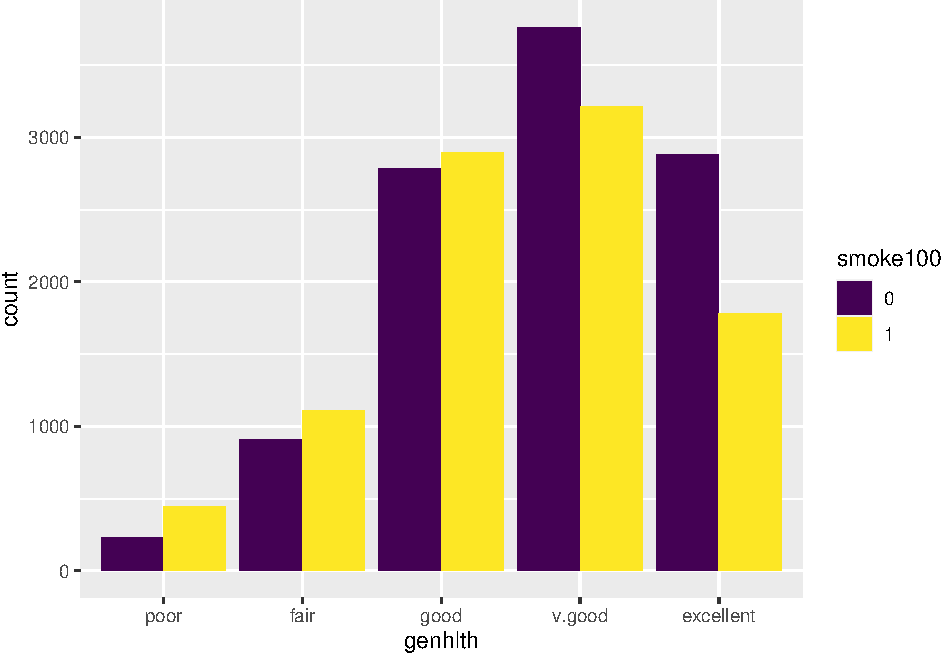
\includegraphics[width=0.5\linewidth]{rj_paper_files/figure-latex/int-pairs-cdcdata-3} 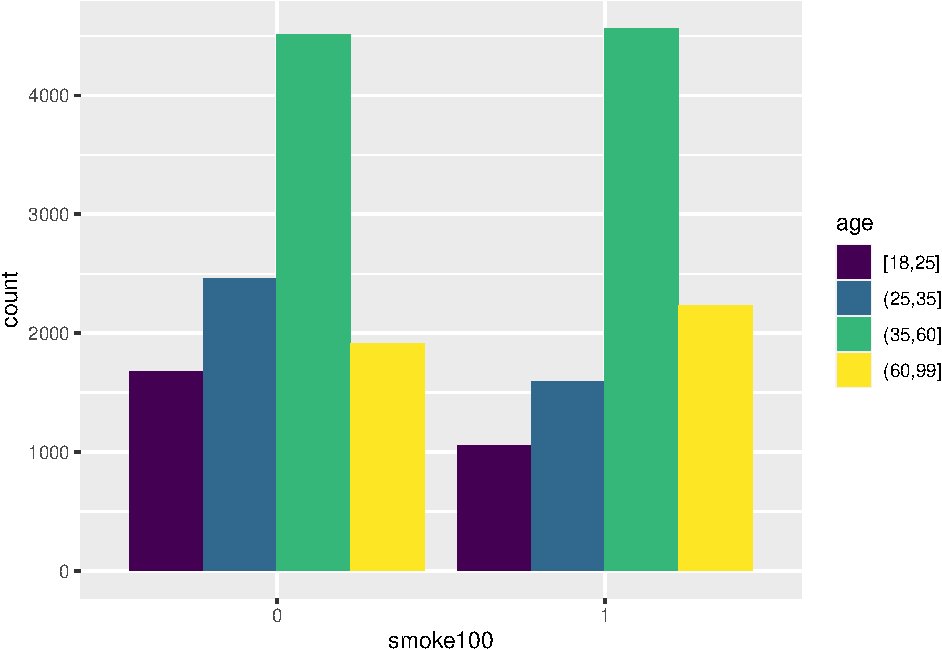
\includegraphics[width=0.5\linewidth]{rj_paper_files/figure-latex/int-pairs-cdcdata-4} \caption[Scatterplot and barplot for numeric variable pair (wtdesire, height) and ordinal variable pairs (genhlth, age), (genhlth,smoke100) and (smoke100, age) showing association between these pair of variables]{Scatterplot and barplot for numeric variable pair (wtdesire, height) and ordinal variable pairs (genhlth, age), (genhlth,smoke100) and (smoke100, age) showing association between these pair of variables.}\label{fig:int-pairs-cdcdata}
\end{figure}
\end{Schunk}

\hypertarget{multiple-association-measures-plot}{%
\subsection{Multiple Association Measures
Plot}\label{multiple-association-measures-plot}}

The multiple association measures plot compares the multiple association
measures for all the variable pairs in a dataset. This display is useful
in detecting variable pairs with high difference among the measures
which then can be explored further in more detail.

\begin{Schunk}
\begin{Sinput}
assoc_german_all <- calc_assoc_all(d = german_election,
                                   measures = c("ace",
                                                "pearson",
                                                "spearman",
                                                "kendall",
                                                "dcor",
                                                "spearman",
                                                "mic"))

plot_assoc_linear(assoc = assoc_german_all, 
                  plot_type = "heatmap",
                  limits = c(0,1),
                  var_order = "max_diff")
\end{Sinput}
\begin{figure}

{\centering 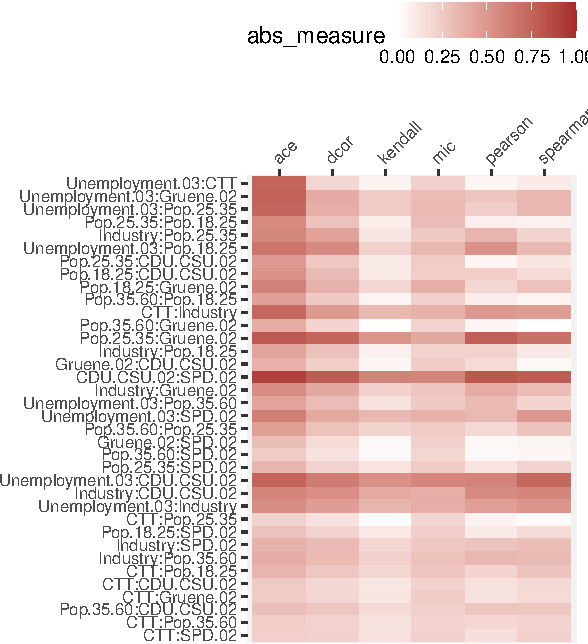
\includegraphics{rj_paper_files/figure-latex/compare-linear-heatmap-1} 

}

\caption[Multiple association measures plot in a linear layout for a subset of German election data]{Multiple association measures plot in a linear layout for a subset of German election data. The plot has variable pairs on the Y-axis and association measures on the X-axis. The color intensity of each cell is proportional to the absolute value of association measure. The variable pairs on Y-axis are ordered by the maximum difference between the absolute value of association measures. The plot shows the highest difference for variable pair V.FDP.02 and V.Linke.02 which can be explored further to understand the underlying reasons for this difference.}\label{fig:compare-linear-heatmap}
\end{figure}
\end{Schunk}

Figure \ref{fig:compare-linear-heatmap} shows a multiple association
measures plot in linear layout for German election dataset. The plot
compares the absolute values of association measures such as
\texttt{ace}, \texttt{dcor}, \texttt{kendall}, \texttt{mic},
\texttt{pearson} and \texttt{spearman} for every variable pair in the
dataset. Each cell of the plot corresponds to a variable pair and an
association measure, and color intensity of each cell corresponds to the
absolute value of association measure. The variable pairs in the plot
are ordered by the maximum difference between the absolute value of
these measures. The plot shows the variable pair
(\texttt{Unemployment.03},\texttt{CTT}) with highest difference between
the association measures. The low value for Pearson's correlation and
Kendall's correlation suggest no trend but measures such as ace,
distance correlation, MIC and Spearman's correlation indicates that a
relationship might exist among the variables. Another interesting
variable pair evident from the plot is (\texttt{Pop.35.60},
\texttt{Gruene.02}) for which the three popular measures like Pearson's,
Kendall's and Spearman's correlation coefficient are almost zero but
measures such as ace, distance correlation and MIC suggest presence of a
pattern.

\begin{Schunk}
\begin{Sinput}
show_assoc(d = german_election,
           x = "Unemployment.03",
           y = "CTT")

show_assoc(d = german_election,
           x = "Gruene.02",
           y = "Pop.35.60")
\end{Sinput}
\begin{figure}
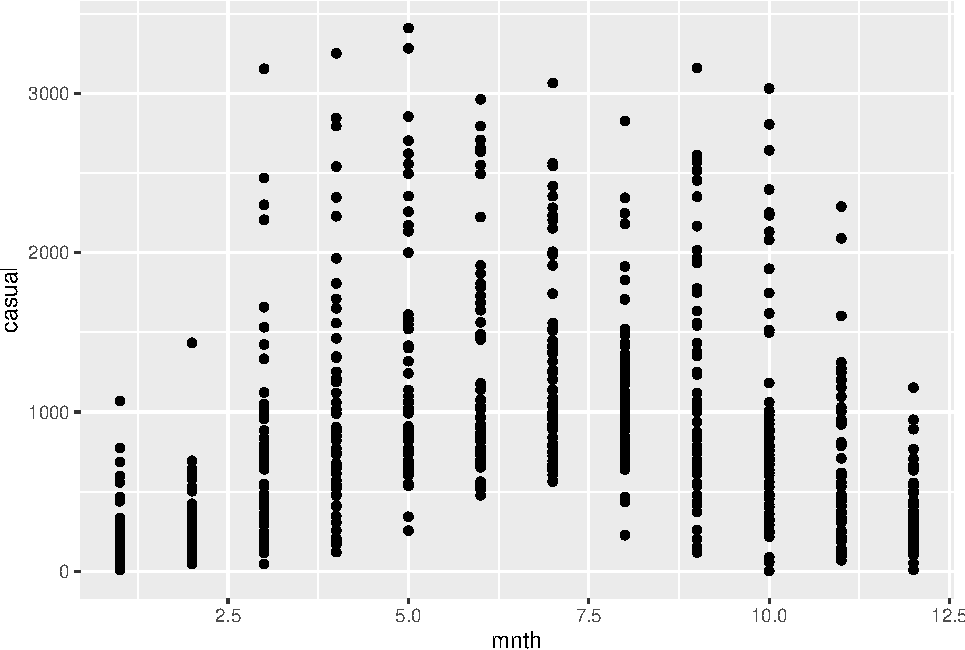
\includegraphics[width=0.5\linewidth]{rj_paper_files/figure-latex/int-pairs-multiple-germanelection-1} 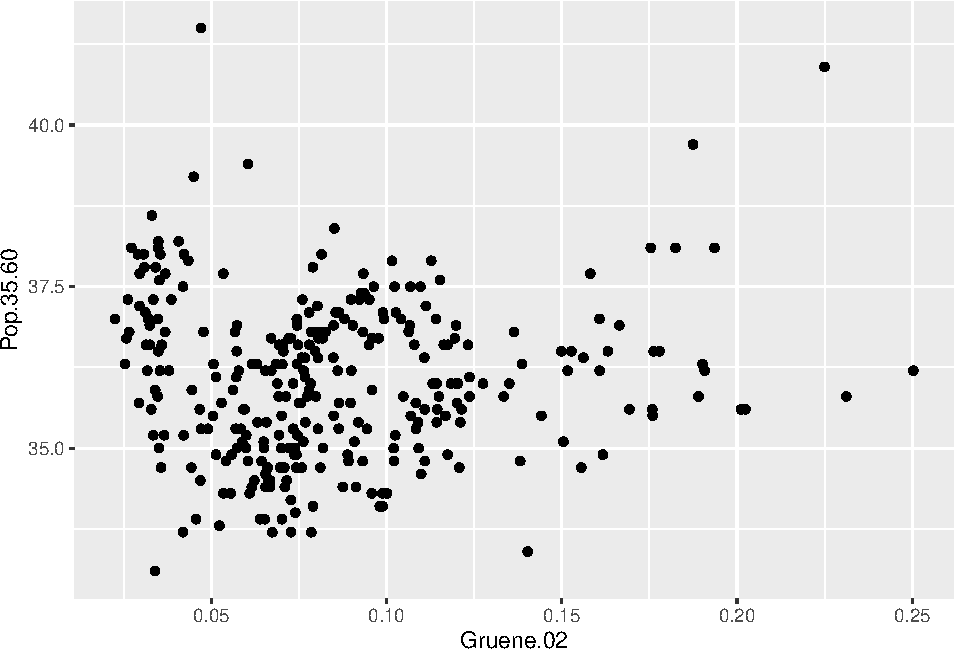
\includegraphics[width=0.5\linewidth]{rj_paper_files/figure-latex/int-pairs-multiple-germanelection-2} \caption[Scatterplot for variable pairs (from left to right) (Unemployment.03 and CTT) and (`Pop.35.60`, `Gruene.02`) showing relationships between these pair of variables]{Scatterplot for variable pairs (from left to right) (Unemployment.03 and CTT) and (`Pop.35.60`, `Gruene.02`) showing relationships between these pair of variables.}\label{fig:int-pairs-multiple-germanelection}
\end{figure}
\end{Schunk}

We use \texttt{show\_assoc} to explore the relationship for the
interesting variable pairs in Figure
\ref{fig:int-pairs-multiple-germanelection}. It is evident from the
plots that the variable pairs (\texttt{Unemployment.03},\texttt{CTT})
and (\texttt{Pop.35.60}, \texttt{Gruene.02}) show a non-linear trend for
which measures such as Pearson's correlation, Kendall's correlation and
Spearman's correlation might not be suitable.

\hypertarget{conditional-association-plot}{%
\subsection{Conditional Association
Plot}\label{conditional-association-plot}}

The conditional association plot is produced by splitting the data by a
partitioning variable and calculating association for the variable pairs
at each level of partitioning variable using \texttt{calc\_assoc}
function with conditioning variable as the \texttt{by} argument. The
calculated association measures are then displayed using bars in a
matrix plot. The height and color of the bars are coded with the value
of association measure and the level of the partitioning variable
respectively. These displays are efficient for discovering variable pair
with high differences among the levels of partitioning variable in the
data.

\begin{Schunk}
\begin{Sinput}
cond_assoc_cdc <- calc_assoc(d = cdcdata, 
                             by = "genhlth")
plot_assoc_matrix(lassoc = cond_assoc_cdc)
\end{Sinput}
\begin{figure}

{\centering 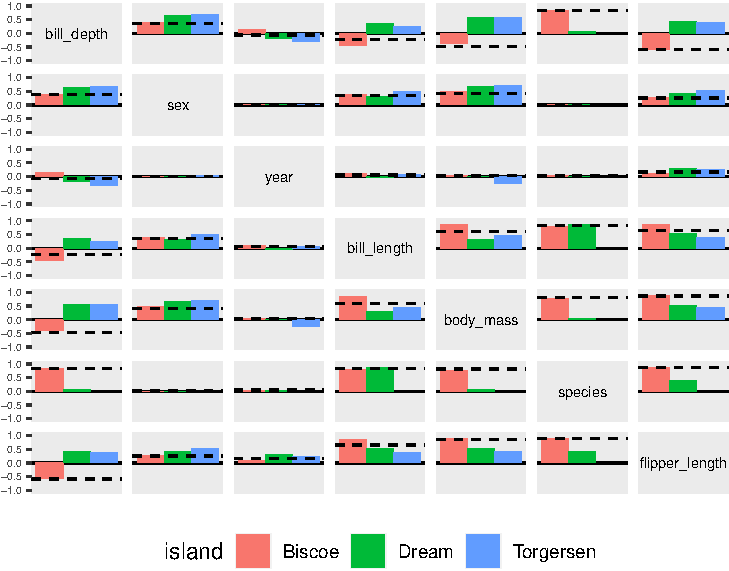
\includegraphics{rj_paper_files/figure-latex/cond-assoc-1} 

}

\caption[Conditional Association plot for cdc data showing Pearson's correlation for numeric pairs, Goodman and Kruskal's gamma for ordinal pair, canonical correlation for nominal or mixed pairs]{Conditional Association plot for cdc data showing Pearson's correlation for numeric pairs, Goodman and Kruskal's gamma for ordinal pair, canonical correlation for nominal or mixed pairs. The bars in each cell represent the value for asssociation measure colored by the conditioning variable genhlth The dotted line in each cell represents overall value of the association measure. The plot shows evident difference in measure value for pair (smoke100, age) and (weight, gender) for participants with different levels of health in the data.}\label{fig:cond-assoc}
\end{figure}
\end{Schunk}

Figure \ref{fig:cond-assoc} shows a conditional association plot for the
cdc data. Each cell corresponding to a variable pair shows two bars
which correspond to the association measure (Pearson's correlation for
numeric pairs, Goodman and Kruskal's gamma for ordinal pair, canonical
correlation for nominal or mixed pairs) calculated at the levels of
conditioning variable \texttt{genhlth}. The dotted line represents the
overall association measure. The plot indicates that there is an evident
difference in the Goodman and Kruskal's gamma for the variable pair
(\texttt{smoke100}, \texttt{age}) for different levels of health,
compared with each other and overall value. Also, the canonical
correlation for variable pair (\texttt{weight}, \texttt{gender}) for
individuals feeling poor or fair health is low compared to the overall
value. We explore these variable pairs in more detail using
\texttt{show\_assoc}.

\begin{Schunk}
\begin{Sinput}
show_assoc(d = cdcdata,
           x = "smoke100",
           y = "age",
           by = "genhlth")

show_assoc(d = cdcdata,
           x = "weight",
           y = "gender",
           by = "genhlth")
\end{Sinput}
\begin{figure}
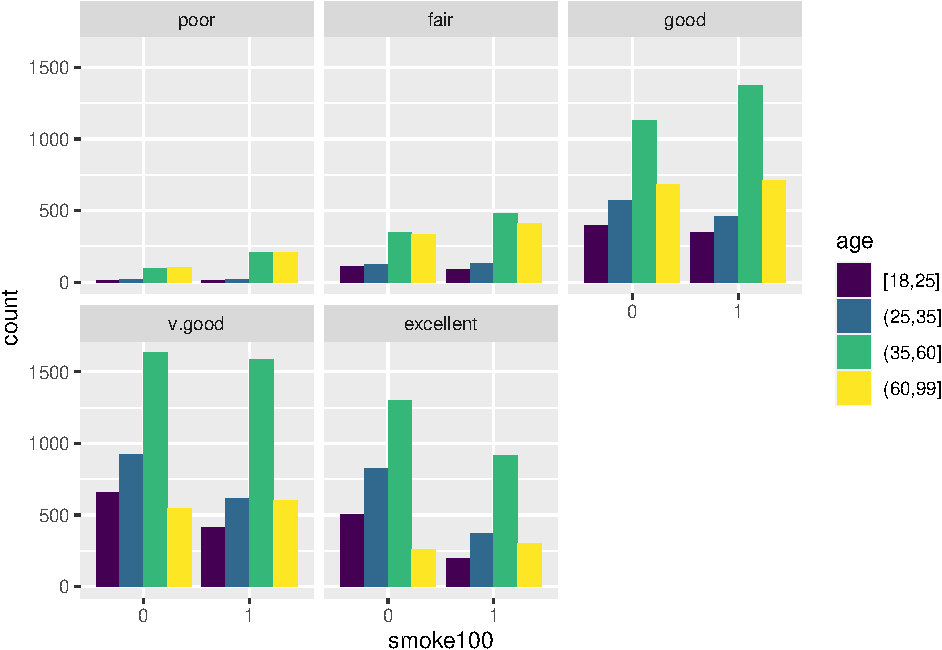
\includegraphics[width=0.5\linewidth]{rj_paper_files/figure-latex/int-pairs-conditional-cdc-1} 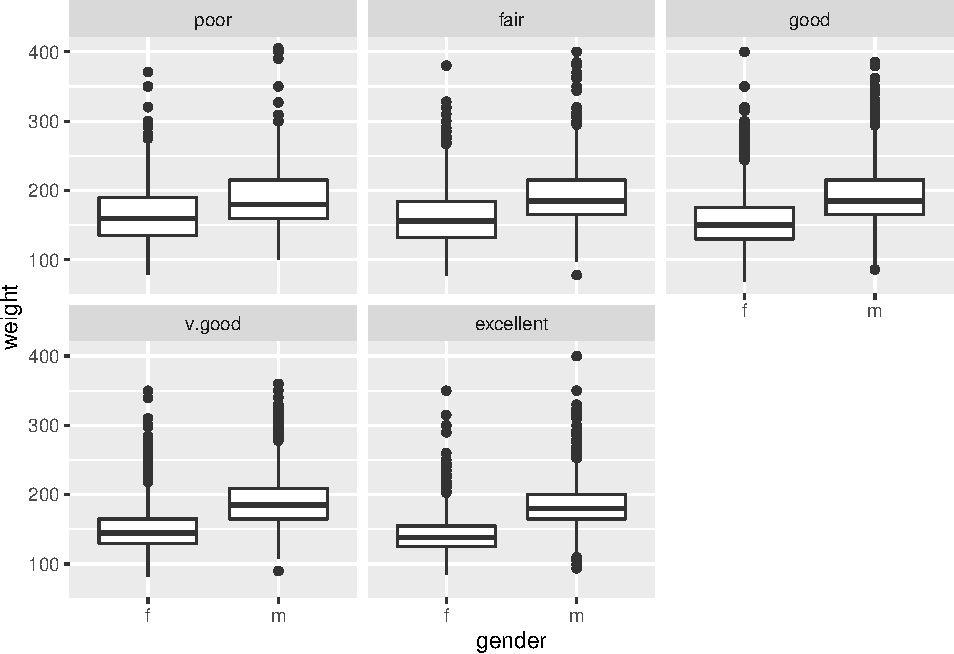
\includegraphics[width=0.5\linewidth]{rj_paper_files/figure-latex/int-pairs-conditional-cdc-2} \caption[Barplot for variable pair (smoke100, age), and boxplot for variable pair (weight, gender) faceted by conditioning variable genhlth]{Barplot for variable pair (smoke100, age), and boxplot for variable pair (weight, gender) faceted by conditioning variable genhlth.}\label{fig:int-pairs-conditional-cdc}
\end{figure}
\end{Schunk}

Figure \ref{fig:int-pairs-conditional-cdc} shows a barplot for the
variable pair (\texttt{smoke100}, \texttt{age}) and a boxplot for
variable pair (\texttt{weight}, \texttt{gender}) faceted by the
conditioning variable \texttt{genhlth}. The faceted barplot shows that
individuals who are old with smoking habits suffer with poor health more
(almost twice) compared to individuals who are old and don't smoke.
Interstingly, the faceted boxplot shows that healthier females have low
weight compared to the females who don't feel healthy. On the other
hand, the weight of the males who feel either health or unhealthy have
fairly similar weight.

We also use linear layouts for displaying conditional association in the
package. The function \texttt{plot\_assoc\_linear} is used for
displaying a linear layout of the conditional association for variable
pairs in the dataset. The association measures are calculated for every
variable pair at each level of partitioning variable using
\texttt{calc\_assoc} function with conditioning variable as the
\texttt{by} argument.

The measures are then displayed using a dotplot (or a heatmap) where
color of the dots (or each cell) is coded by the level of the
partitioning variable and the variable pairs are ordered by absolute
maximum value of association measure for each of the pair of variable.
These displays are also efficient for discovering differences among the
levels of partitioning variable in the data. In comparison to matrix
layout, it is easier to omit less relevant pairs of variables in linear
layouts by filtering the variables pairs having a higher value for
association measures than a threshold.

Figure \ref{fig:linear-cond-assoc} shows a linear display for
conditional association measures with the variable pairs having absoulte
measure value greater than \(0.1\) along the Y-axis, the value of
association measure along X-axis and color of the points representing
the level of the grouping variable. The linear layout becomes more
useful over the matrix layout for conditional association display when
the number of variables and number of levels of grouping variable are
high.

\begin{Schunk}
\begin{Sinput}
cond_assoc_cdc <- calc_assoc(d = cdcdata, 
                             by = "genhlth")
cond_assoc_cdc <- dplyr::filter(cond_assoc_cdc, abs(measure) > 0.1)
plot_assoc_linear(assoc = cond_assoc_cdc,
                  plot_type = "dotplot")
\end{Sinput}
\begin{figure}

{\centering 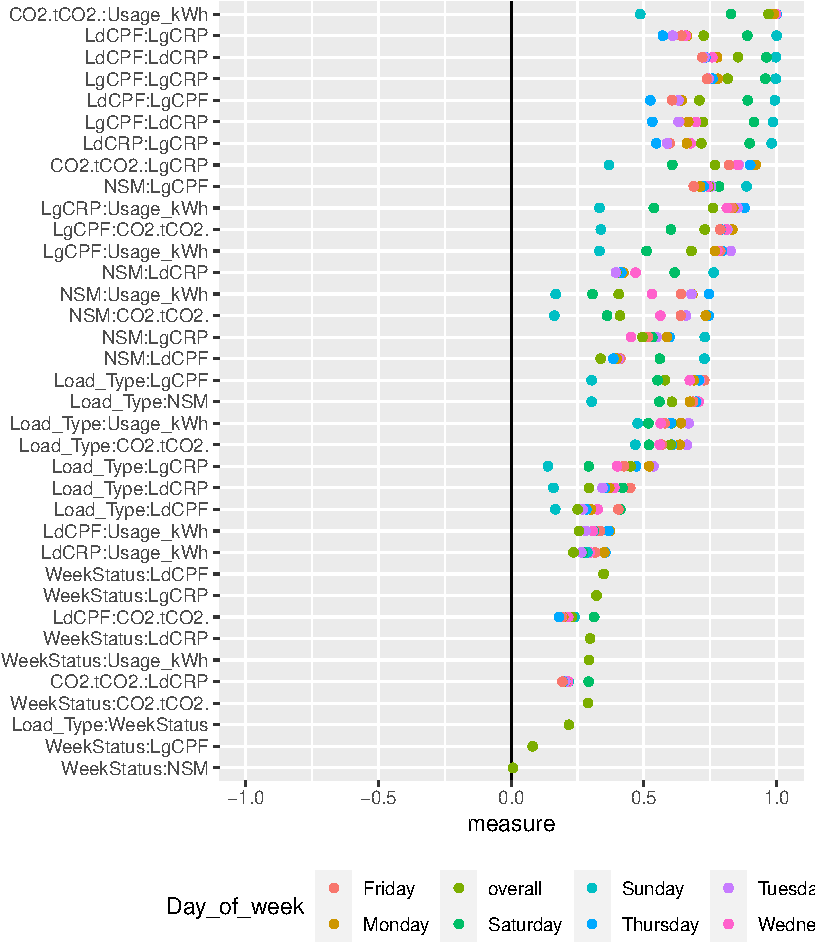
\includegraphics{rj_paper_files/figure-latex/linear-cond-assoc-1} 

}

\caption[Conditional Association plot using linear layout.The display has variable pairs on the Y-axis and the value of association measures on the X-axis]{Conditional Association plot using linear layout.The display has variable pairs on the Y-axis and the value of association measures on the X-axis. The points corresponding to every variable pair represents the value of association measure for different levels of the conditioning variable and the overall value of association measure.}\label{fig:linear-cond-assoc}
\end{figure}
\end{Schunk}

\hypertarget{section-5-discussion}{%
\section{Section 5: Discussion}\label{section-5-discussion}}

We use multiple association measures in a single display for different
variable pairs which serves as a comparison tool while exploring
association in a dataset and assist in identifying unusual variable
pairs. These multiple measures can be displayed in a scatterplot matrix
similar to what \citet{tukey1985computer} proposed. They suggested that
scatterplot matrix of the scagnostics measures, which are measures
summarizing a scatterplot, can be used to identify unusual scatterplots
or variable pairs. \citet{wilkinson2005graph} used this idea with their
graph-theoretic scagnostic measures to highlight unusual scatterplots.
Similarly, \citet{kuhn2013applied} have used this idea in a predictive
modeling context. They have produced a scatterplot matrix of the
measures between the response and continuous predictors such as
Pearson's correlation coefficient, pseudo-\(R^2\) from the locally
weighted regression model, MIC and Spearman's rank correlation
coefficient to explore the predictor importance during feature selection
step. These displays show the importance of comparing multiple
association measures at once for different variable pairs.

\bibliography{RJreferences.bib}

\address{%
Amit Chinwan\\
Maynooth University\\%
Hamilton Institute\\ Maynooth, Ireland\\
%
%
%
\href{mailto:amit.chinwan.2019@mumail.ie}{\nolinkurl{amit.chinwan.2019@mumail.ie}}%
}

\address{%
Catherine Hurley\\
Maynooth University\\%
Department of Mathematics and Statistics\\ Maynooth, Ireland\\
%
%
%
\href{mailto:catherine.hurley@mu.ie}{\nolinkurl{catherine.hurley@mu.ie}}%
}
